\chapter{Implementation}
\label{ch:Implementation}

This chapter describes the theoretical design of the filter algorithm proposed in \cite{bennett_motion_2014}, as well as its implementation, based on the fundamentals acquired in the previous chapters. Other than \citeauthor{bennett_motion_2014} in \cite{bennett_motion_2014} who tested the filter algorithm by hand, we used movement data from real subjects. After outlining the initial situation, i.\,e. stating existing orientation algorithms, the theoretical design of the filter is described in detail. Subsequently, the software implementation and experiments are given, followed by the results and its discussion.

\section{Initial Situation}

There were already a variety of Kalman filter algorithms implemented. In tandem with an orientation estimation based on a Qualisys motion capture system using cameras in combination with optical markers, they served as a reference. The placement of the markers on the leg are depicted in Figure \ref{fig:marker_placement}. From the recorded motion of the markers in space the motion capture system computed the orientation angles of the thighs and shanks.

(Any algorithms that are already implemented for comparison that I can cite or state and describe how they differ from the one that I will implement??)

\begin{figure}
\centering
	\begin{tikzpicture}[auto, thick, node distance=3cm,>=latex']
    \pgftext{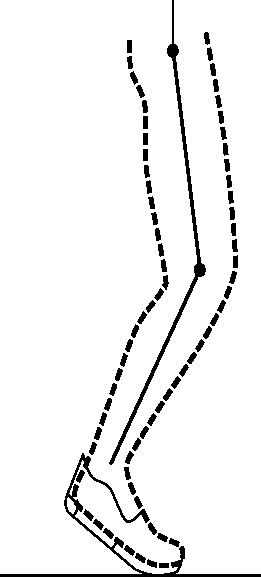
\includegraphics[width=3.5cm]{images/sensors_on_leg}} at (0pt,0pt);
    \node [] (a) at (-4.4, -2) {};
    \node [] (b) at (-4.5, 0.1) {};
    \node [] (c) at (4.45, 3.3) {};
\end{tikzpicture}
\caption{Human leg with optical markers, from \cite{tao_gait_2012}.} \label{fig:marker_placement}
\end{figure} 

\section{Theoretical Design}\label{sec:theoretical_design}

This section maps the theoretical design of the system proposed by \citeauthor{bennett_motion_2014} in \cite{bennett_motion_2014} to the existing GaitWatch system. It states the assigned coordinate frames and the conventions with respect to rotation about them. Furthermore, it describes the kinematic model and the extended Kalman filter in detail.

\subsection{Kinematic model}

The \emph{kinematic model} relates the respective angles of the thigh and shank about the hip and knee joint to the acceleration seen by the wearable sensors. When walking in a straight line, the human leg can be modelled as a two-link planar revolute robot \cite{bennett_motion_2014}. Then, thighs and shanks remain in a single plane which is approximately parallel to the direction of motion. As depicted in Figure \ref{fig:robot}, the revolute joints of the \gls{pendubot} represent the hip und knee joint, and the two links the thigh and shank, respectively. The origin of the inertial world frame is located at the base of link 1, the upper of both links. The $x$-axis points forward, the $y$-axis points out from the hip to the right, and the $z$-axis points down. Thus, since the figure depicts the right leg from lateral, the $y$-axis points out of the page. This configuration follows the right-hand rule, which can also be used to determine the sense of rotation around the axes. The pitch angle $\theta_1$ is measured with respect to the $x$-axis, and the pitch angle $\theta_2$ of link 2, with respect to link 1. 

\begin{figure}
\centering
\begin{tikzpicture}[auto, thick,>=latex']
	\node [draw, rectangle, minimum height=1.6cm, minimum width=1.6cm, pattern=north west lines] at (0,0) (solid) {};

    \node [draw,  fill=white, very thick, rectangle, rounded corners=3pt, minimum height=3.7cm, minimum width=1cm, align=center, rotate around={30:(0,0)}] at (0.7, -1.25) (link1) {};
    \node [draw, thick, fill=gray, rounded corners=2pt, rectangle, minimum height=0.8cm, minimum width=0.5cm, align=center, rotate around={30:(0, 0)}, label={[label distance=0.18cm]335:IMU 1}] at (0.98, -1.7) (sensor1) {};
    
    \node [draw, fill=white, very thick, rectangle, rounded corners=3pt, minimum height=3.7cm, minimum width=0.6cm, align=center, rotate around={145:(0,0)}] at (0.6, -3.7) (link2) {};
    \node [draw, thick, fill=gray, rounded corners=2pt, rectangle, minimum height=0.8cm, minimum width=0.5cm, align=center, rotate around={145:(0, 0)}, label={right:IMU 2}] at (0, -4.56) (sensor2) {};
    
    \node[coordinate] (X) at (2.5,0) {};
    \node[coordinate] (Y) at (0,-2.5) {};
    \node[coordinate] (O) at (-0, 0) {};
    
    \draw[->] (O) -- node[name=x] {$x$}(X);
    \draw[->] (O) -- node[pos=0.6, name=y, label={left:$z$}] {}(Y);
    
    \draw[->] (0, -4.56) -- node[name=x_2] {$x_2$}(1.5, -5.6);
    \draw[->] (0, -4.56) -- node[name=x_2] {$z_2$}(-1.1, -6.1);
   
    \draw[dotted] (O) -- (2.5,-4.3);
    \draw[fill=white] (0,0) circle (4pt);
    \draw[fill=black] (0,0) circle (1pt) node[label={[label distance=-1.2mm]180:$y$}]{};
    \draw (1.45, -2.5) circle (4pt);
    
    \draw[-stealth] (1.2,-1) arc (300:355:1.2);
    \draw[-stealth] (0.8,-4.1) arc (240:303:1.4);
    
    \node at (1.3, -0.4) (angle1) {$\theta_1$};
    \node at (1.5, -3.7) (angle1) {$\theta_2$};
\end{tikzpicture}
\caption{Kinematic model of the human leg, from \cite{bennett_motion_2014}.} \label{fig:robot}
\end{figure} 

The \glspl{IMU} placed on the thighs and shanks measured the angular velocity and linear acceleration of the thighs and shanks, respectively. According to \citeauthor{spong2005robot} \cite{spong2005robot}, the $x$ and $z$ displacement and its derivatives in the world frame are as follows:

\begin{align}
  x &= a_1 \cos \theta_1 + a_2 \cos(\theta_1 + \theta_2) \\
  \dot{x} &= -a_1 \dot{\theta}_1 \sin \theta_1  - a_2 (\dot{\theta}_1 + \dot{\theta}_2) \sin(\theta_1 + \theta_2) \\
  \ddot{x} {}&= -a_1 [\dot{\theta}^2_1 \cos \theta_1 + \ddot{\theta}_1 \sin \theta_1] - a_2 [(\dot{\theta}_1 + \dot{\theta}_2)^2 \cos(\theta_1 + \theta_2) \nonumber \\ 
  &\mathrel{\phantom{=}} + (\ddot{\theta}_1 + \ddot{\theta}_2) \sin(\theta_1 + \theta_2)] \label{eq:acc_x} \\
  \nonumber \\
  z &= -a_1 \sin \theta_1 - a_2 \sin(\theta_1 + \theta_2) \\
  \dot{z} &= -a_1 \dot{\theta}_1 \cos \theta_1  - a_2 (\dot{\theta}_1 + \dot{\theta}_2) \cos(\theta_1 + \theta_2) \\
  \ddot{z} {}&= -a_1 [\ddot{\theta}_1 \cos \theta_1 - \dot{\theta}^2_1 \sin \theta_1] - a_2 [(\ddot{\theta}_1 + \ddot{\theta}_2) \cos(\theta_1 + \theta_2) \nonumber \\ 
  &\mathrel{\phantom{=}} + (\dot{\theta}_1 + \dot{\theta}_2)^2 \sin(\theta_1 + \theta_2)] \label{eq:acc_y}
\end{align}

\noindent
in which $a_1$ and $a_2$ are the lengths of the two links, respectively. Using Equations \ref{eq:acc_x} and \ref{eq:acc_y}, and the estimates of the angles $\theta_1$ and $\theta_2$ and their derivatives obtained with the EKF described in Section \ref{sec:EKF_model} we can estimate the motion based acceleration in $x$ and $z$ direction that sensor 2 will see in the world coordinate frame.

The orientation of the sensor frames at rest are different from the world frame and dynamic when the pendulum is in motion. In order to transform the values from the world frame to the dynamic body frame of \gls{IMU} 2, which is seen in Figure \ref{fig:robot}, we used the transformation matrix $\mathbf{T}_y(\theta)$ from Equation \ref{eq:transformation_matrices} in transposed form. The positive sense of rotation according the right-hand rule is opposite to the mathematically positive sense, which is why we use the transpose of the transformation matrix. The body frame of sensor two is not aligned with the world frame for $\theta_1 = \theta_2 = 0$. Thus, an offset of $-\frac{\pi}{2}$ is necessary. With $\theta = \theta_1 + \theta_2 - \frac{\pi}{2}$, this yields

\begin{equation}
\mathbf{T}^T_y(\theta_1 + \theta_2 - \frac{\pi}{2}) = \begin{bmatrix}
    \cos (\theta_1 + \theta_2 - \frac{\pi}{2}) \; & 0 \; & \sin (\theta_1 + \theta_2 - \frac{\pi}{2}) \\
    0 \; & 1 \; & 0 \\
    -\sin (\theta_1 + \theta_2 - \frac{\pi}{2}) \; & 0 \; & \cos (\theta_1 + \theta_2 - \frac{\pi}{2})
    \end{bmatrix}\,.
\end{equation}

\noindent
The rotated tangential and radial components of the motion based acceleration estimates, $A_{rad}$ and $A_{tan}$ are found using the tranformation matrix to rotate the results of Equations \ref{eq:acc_x} and \ref{eq:acc_y}, respectively, according to Equation \ref{eq:transformation}.

\begin{equation}
  A_{rad} = \mathbf{T}^T_y(\theta_1 + \theta_2 - \frac{\pi}{2}) \ddot{x}
\end{equation}

\begin{equation}
  A_{tan} = \mathbf{T}^T_y(\theta_1 + \theta_2 - \frac{\pi}{2}) \ddot{z}
\end{equation}

Then, the radial and tangential acceleration estimates are subtracted from the sensor readings $A_x$ and $A_y$, which leaves an estimate of the gravity based acceleration $\mathbf{g}$ that acts on the sensor:

\begin{equation}
\mathbf{g} = \begin{bmatrix}
    g_x \\
    g_y 
    \end{bmatrix} = 
    \begin{bmatrix}
    A_x \\
    A_z 
    \end{bmatrix} -
    \begin{bmatrix}
    A_{rad} \\
    A_{tan} 
    \end{bmatrix}\,.
\end{equation}

\noindent
According to Equation \ref{eq:projection_gravity} the angle estimate is

\begin{equation}
  \theta_1 + \theta_2 = \mbox{atan}2(g_y, g_x)\,.
\end{equation}

\noindent
This improved angle estimate is then fused with the estimate based on the integration of the angular rate measured with the gyroscope, in order to reduce the estimation error due to gyroscope drift.

\subsection{Extended Kalman Filter Model}\label{sec:EKF_model}

The state-space model of the extended Kalman filter is given by the state vector $\mathbf{x} \in \mathbb{R}^{n=10}$

\begin{equation} \label{eq:state_vector}
  \mathbf{x} = \begin{bmatrix}
  	x, & z, & \theta_1, & \omega_1, & \alpha_1, & \theta_2, & \omega_2, & \alpha_2, & \beta_1, & \beta_2
  \end{bmatrix}^T
\end{equation}

\noindent
where $x$ and $y$ correspond to the horizontal and vertical position of the end of link 2 with respect to the origin of the world frame, i.\,e. the hip joint. $\theta_1$ is the angle, $\omega_1$ the angular velocity, and $\alpha_1$ the angular acceleration of the first joint, respectively. The corresponding values for the second link are $\theta_2$, $\omega_2$, and $\alpha_2$. The biases from the gyroscope on the first and second sensor are $\beta_1$ and $\beta_2$, respectively. They are assumed to be constant or slowly time varying.

The measurement vector $\mathbf{z} \in \mathbb{R}^{m=3}$ is given by

\begin{equation} \label{eq:measurement_vector}
  \mathbf{z} = \begin{bmatrix} z_1 \\ z_2 \\ z_3 \end{bmatrix} = \begin{bmatrix}
  	\omega_1 + \beta_1, & \omega_1 + \omega_2 + \beta_2, & \theta_1 + \theta_2
  \end{bmatrix}^T + \mathbf{v}\,.
\end{equation}
 
\noindent
where $\mathbf{v}$ is the random measurement noise process, modelled as zero-mean, Gaussian white noise. The element $z_1$ represents the measurement of the first link angular velocity, which is the sum of the first link rotation and the gyroscope 1 bias. Equally, the element $z_2$ represents the measurement of the second link angular velocity, which is the sum of the first and second link rotation and the bias of gyroscope 2. Finally, the element $z_3$ is the angle estimate of the second accelerometer, which will see the angular displacement of both links.

The plant dynamics of the modelled system can be expressed as a set of $n$ coupled first-order ordinary differential equations \cite{rowell2002state}, in which the time derivative of each state variable is expressed in terms of the state variables $x_1(t), \dots, x_n(t)$. These equations are known as the \emph{state equations}. The modelled system is governed by the \emph{non-linear} ordinary differential equations

\begin{equation} \label{eq:state_vector_derivative}
  \dot{\mathbf{x}} = \mathbf{f}(\mathbf{x}, t) + \mathbf{w} = \left[\begin{smallmatrix}
  -a_1 \omega_1 \sin \theta_1  - a_2 (\omega_1 + \omega_2) \sin(\theta_1 + \theta_2) \\
  -a_1 \omega_1 \cos \theta_1  - a_2 (\omega_1 + \omega_2) \cos(\theta_1 + \theta_2) \\ \omega_1 \\ \alpha_1 \\ 0 \\ \omega_2 \\ \alpha_2 \\ 0 \\ 0 \\ 0
  \end{smallmatrix}\right] + \mathbf{w}\,,
\end{equation}

\noindent
where the components of $\mathbf{f}(\mathbf{x},t)$, that is $f_i(\mathbf{x})$ are the component-wise time derivatives $\dot{x}_i = \frac{dx_i}{dt}$, $i = 1, \dots, n$ of the state vector $\mathbf{x}$. Given this notation, the system state at any instant may be interpreted as a point in an $n$-dimensional state space whose axes are the state variables. The dynamic state response $\mathbf{x}(t)$ can be interpreted as a trajectory traced out in the state space.

The state equation can be written in state-space form as 

\begin{equation}
  \dot{\mathbf{x}} = \mathbf{F} \mathbf{x} + \mathbf{w}\,,
\end{equation}

\noindent
where the system dynamics matrix $\mathbf{F}$ is the Jacobian of $\mathbf{f}(\mathbf{x},t)$, given by

\begin{equation}
\begin{split}
\mathbf{F} = \mathbf{J}_{\mathbf{f}} |_{\mathbf{x}=\hat{\mathbf{x}}_{k-1}} &= \begin{bmatrix}
    \dfrac{\partial f_1}{\partial x_1} & \cdots & \dfrac{\partial f_1}{\partial x_{n}}\\
    \vdots & \ddots & \vdots\\
    \dfrac{\partial f_{n}}{\partial x_1} & \cdots & \dfrac{\partial f_{n}}{\partial x_{n}} \end{bmatrix}_{\mathbf{x}=\hat{\mathbf{x}}_{k-1}} \\
&=\begin{bmatrix}
  0 & 0 & 0 & A & 0 & 0 & B & 0 & 0 & 0\\
  0 & 0 & 0 & C & 0 & 0 & D & 0 & 0 & 0\\
  0 & 0 & 0 & 1 & 0 & 0 & 0 & 0 & 0 & 0\\
  0 & 0 & 0 & 0 & 1 & 0 & 0 & 0 & 0 & 0\\
  0 & 0 & 0 & 0 & 0 & 0 & 0 & 0 & 0 & 0\\
  0 & 0 & 0 & 0 & 0 & 0 & 1 & 0 & 0 & 0\\
  0 & 0 & 0 & 0 & 0 & 0 & 0 & 1 & 0 & 0\\
  0 & 0 & 0 & 0 & 0 & 0 & 0 & 0 & 0 & 0\\
  0 & 0 & 0 & 0 & 0 & 0 & 0 & 0 & 0 & 0\\
  0 & 0 & 0 & 0 & 0 & 0 & 0 & 0 & 0 & 0\\
\end{bmatrix}_{\mathbf{x}=\hat{\mathbf{x}}_{k-1}}\,,
\end{split}
\end{equation}

\noindent
and

\begin{equation*}
  \begin{array}{cc}
  \begin{split}
  	A &= -a_1 \sin \theta_1 -a_2 \sin (\theta_1 + \theta_2)\,, \quad \\
  	C &= a_1 \cos \theta_1 + a_2 \cos (\theta_1 + \theta_2)\,,
  \end{split} &
  \begin{split}
  B &= -a_2 \sin (\theta_1 + \theta_2)\,, \\
  C &= a_2 \cos (\theta_1 + \theta_2)\,.
  \end{split}
\end{array}
\end{equation*}

\noindent
The partial derivatives are evaluated at the current state estimates $\hat{\mathbf{x}}_{k-1}$.

As outlined in \cite{zarchan2009fundamentals}, the \emph{fundamental matrix} $\bm{\Phi}(t)$ that propagates the state of the system forward from any time $t_0$ to a time $t$ can be found by a Taylor-series expansion 

\begin{equation}
  \bm{\Phi}(t-t_0) = \mathbf{I} + \mathbf{F} (t-t_0) + \frac{\mathbf{F}^2 (t-t_0)^2}{2!} +\frac{\mathbf{F}^{3} (t-t_0)^3}{3!} + \cdots.
\end{equation}
 
\noindent
The linear approximation of the fundamental matrix yields

\begin{equation}
  \bm{\Phi}^{[1]}(t-t_0) \approx \mathbf{I}_n + \mathbf{F} (t-t_0)\,.
\end{equation}

\noindent
Therefore, the discrete fundamental matrix can be found by substituting $T_s$ for $t-t_0$

\begin{equation}
  \bm{\Phi}^{[1]}_{k} \approx \mathbf{I}_{n} + \mathbf{F} T_s\,.
\end{equation}

\noindent
where $T_s$ is the sampling period and $\mathbf{I} \in \mathbb{R}^{10 \times 10}$ the identity matrix. 

The estimate $\hat{\mathbf{x}}_{k-1}$ can be propagated forward to the \emph{a priori} estimate $\hat{\mathbf{x}}^{-}_k$ by integrating the non-linear differential equation at each sampling interval. Applying Euler integration Equation \ref{eq:apriori_estimate_extended} yields

\begin{equation}\label{eq:apriori_estimate_extended_model}
\begin{split}
	\hat{\mathbf{x}}^{-}_k &= \bm{\phi}_{k-1}(\mathbf{x}_{k-1}, 0) \\
	&= \hat{\mathbf{x}}_{k-1} + \mathbf{f}(\hat{\mathbf{x}}_{k-1}, kT_s)T_s
\end{split}  
\end{equation}

\noindent
where $T_s$ is the integration interval. The control input $\mathbf{u}_k$ is equal to zero since the system does not have any inputs.

The relation between the states and the measurements is linear. The measurement matrix $\mathbf{H} \in \mathbb{R}^{3 \times 10}$ according to Equation \ref{eq:time_dynamical_system_measurement} is given by 

\begin{equation}
\mathbf{H} = \begin{bmatrix}
  0 & 0 & 0 & 1 & 0 & 0 & 0 & 0 & 1 & 0\\
  0 & 0 & 0 & 1 & 0 & 0 & 1 & 0 & 0 & 1\\
  0 & 0 & 1 & 0 & 0 & 1 & 0 & 0 & 0 & 0\\
\end{bmatrix}\,.
\end{equation}

The process and measurement covariance matrices $\mathbf{Q} \in \mathbb{R}^{10 \times 10}$ and $\mathbf{R} \in \mathbb{R}^{3 \times 3}$, respectively, are given by

\begin{equation}
\mathbf{Q} = \begin{bmatrix}
  \sigma_d & 0 & 0 & 0 & 0 & 0 & 0 & 0 & 0 & 0\\
  0 & \sigma_d & 0 & 0 & 0 & 0 & 0 & 0 & 0 & 0\\
  0 & 0 & \frac{\sigma^9_{\theta 1}}{9} & \frac{\sigma^4_{\theta 1}}{4} & \frac{\sigma^5_{\theta 1}}{5} & 0 & 0 & 0 & 0 & 0\\
  0 & 0 & \frac{\sigma^4_{\theta 1}}{4} & \frac{\sigma^3_{\theta 1}}{3} & \frac{\sigma^2_{\theta 1}}{2} & 0 & 0 & 0 & 0 & 0\\
  0 & 0 & \frac{\sigma^5_{\theta 1}}{5} & \frac{\sigma^2_{\theta 1}}{2} & \sigma_{\theta 1} & 0 & 0 & 0 & 0 & 0\\
  0 & 0 & 0 & 0 & 0 & \frac{\sigma^9_{\theta 2}}{9} & \frac{\sigma^4_{\theta 2}}{4} & \frac{\sigma^5_{\theta 2}}{5} & 0 & 0\\
  0 & 0 & 0 & 0 & 0 & \frac{\sigma^4_{\theta 2}}{4} & \frac{\sigma^3_{\theta 2}}{3} & \frac{\sigma^2_{\theta 2}}{2} & 0 & 0\\
  0 & 0 & 0 & 0 & 0 & \frac{\sigma^5_{\theta 2}}{5} & \frac{\sigma^2_{\theta 2}}{2} & \sigma_{\theta 2} & 0 & 0\\
  0 & 0 & 0 & 0 & 0 & 0 & 0 & 0 & \sigma_{\beta} & 0\\
  0 & 0 & 0 & 0 & 0 & 0 & 0 & 0 & 0 & \sigma_{\beta}\\
\end{bmatrix}\,.
\end{equation}

\begin{equation}
\mathbf{R} = \begin{bmatrix}
  \sigma_1 & 0 & 0\\
  0 & \sigma_2 & 0\\
  0 & 0 & \sigma_3
\end{bmatrix}\,,
\end{equation}

\noindent
The process noise matrix $\mathbf{Q}$ is constant. The parameters $\sigma_d, \sigma_{\theta 1}, \sigma_{\theta 2}$ and $\sigma_{\beta}$ are determined by tuning for the best performance. The elements $\sigma_1$ and $\sigma_2$ of $\mathbf{R}$ are constant. They are determined by computing the sample standard deviation of the measurement data during an initialisation stage while the subject stands still. The standard deviation of a finite data set with $n$ samples $x_1, x_2, \dots, x_n$ is

\begin{equation}
  \sigma = \sqrt{\frac{1}{n-1} \sum_{i=1}^n (x_i - \mu)^2}, {\rm \ \ where\ \ } \mu = \frac{1}{n} \sum_{i=1}^n x_i\,.
\end{equation}

\noindent
The standard deviation $\sigma_3$ is set dynamically based on the motion intensity. It toggles between $\sigma_s$ and $\sigma_f$ according to slow or fast motion, distinguished by a threshold $\delta$:

\begin{equation}
  \sigma_3 = \begin{pmatrix}
  	\sigma_s & < \delta\\
  	\sigma_f & \mbox{else}
  \end{pmatrix}
\end{equation}

In order to determine the motion intensity we used the \gls{LTSD} developed in \cite{olivares_vicente_gaitwatch_2013}. The \gls{LTSD} computes the long term spectral envelope of the signal.

\subsection{Summary of the Entire Filter Algorithm}

The state estimates are computed recursively according to the \emph{time update} Equations \ref{eq:apriori_error_cov_extended}, \ref{eq:apriori_estimate_extended_model} and the \emph{measurement update} Equations \ref{eq:aposteriori_estimate}, \ref{eq:Kalman_gain}, and \ref{eq:aposteriori_error_cov}. The entire computation steps of the recursive filter algorithm are summarised in Figure \ref{fig:entire_filter_algorithm}.

\tikzstyle{block} = [draw, rectangle, thick, 
    minimum height=1.5cm, minimum width=9cm]
\tikzstyle{output} = [coordinate]

\begin{figure}
\centering
\begin{tikzpicture}[scale=0.95, every node/.style={transform shape}, auto, rounded corners=1pt, node distance=5cm,>=latex']
    
\node [block, align=center] (init) {Initialisation of parameters \\[2mm]  $\mathbf{x}_{0}, \mathbf{P}_{0}, \mathbf{H}, \bm{\Phi}^{[1]}_{0}, \mathbf{Q}, \mathbf{R}_{0},$};
\node [block, align=center, below of=init, node distance=3.8cm] (predict) {\emph{Time update} \\[2mm] Compute fundamental matrix: \\ $\bm{\Phi}^{[1]}_{k} \approx \mathbf{I}_{n} + \mathbf{F} T_s$ \\ Compute \emph{a priori} estimate: \\ $\hat{\mathbf{x}}^{-}_k = \hat{\mathbf{x}}_{k-1} + \mathbf{f}(\hat{\mathbf{x}}_{k-1}, kT_s)T_s$ \\ Compute \emph{a priori} error covariance: \\ $\mathbf{P}^-_{k} = \bm{\Phi}^{[1]}_{k-1} \mathbf{P}_{k-1} \bm{\Phi}^{[1]T}_{k-1} + \mathbf{Q}_{k-1}$};
\node [block, align=center, below of=predict, node distance=6.65cm] (measurement) {\emph{Correct sensor readings} \\[2mm] Compute acceleration due to motion: \\ $\ddot{x} = -a_1 [\omega^2_1 \cos \theta_1 + \alpha_1 \sin \theta_1] - a_2 [(\omega_1 + \omega_2)^2$ \\ $\mathrel{\phantom{=}}\cdot \cos(\theta_1 + \theta_2) + (\alpha_1 + \alpha_2) \sin(\theta_1 + \theta_2)]$ \\ $\ddot{z} = -a_1 [\alpha_1 \cos \theta_1 - \omega^2_1 \sin \theta_1] - a_2 [(\alpha_1 + \alpha_2)$ \\ $\mathrel{\phantom{=}} \cdot \cos(\theta_1 + \theta_2) + (\omega_1 + \omega_2)^2 \sin(\theta_1 + \theta_2)]$ \\ Rotate acceleration to body frame: \\ $A_{rad} = \mathbf{T}^T_y(\theta_1 + \theta_2 - \frac{\pi}{2}) \ddot{x}$ \\ $A_{tan} = \mathbf{T}^T_y(\theta_1 + \theta_2 - \frac{\pi}{2}) \ddot{z}$ \\ Compute gravity estimate: \\ $\mathbf{g} = \begin{bmatrix}
    g_x \\
    g_y 
    \end{bmatrix} = 
    \begin{bmatrix}
    A_x \\
    A_z 
    \end{bmatrix} -
    \begin{bmatrix}
    A_{rad} \\
    A_{tan} 
    \end{bmatrix}$ \\ Compute corrected angle estimate: \\ $\theta_1 + \theta_2 = \mbox{atan}2(g_y, g_x)$};
\node [block, align=center, below of=measurement, node distance=6.6cm] (update) {\emph{Measurement update} \\[3mm] Compute Kalman gain: \\ $\mathbf{K}_{k} = \mathbf{P}^-_k \mathbf{H}^T_k[\mathbf{H}_k \mathbf{P}^-_k \mathbf{H}^T_k + \mathbf{R}_k]^{-1}$ \\ Compute \emph{a posteriori} estimate: \\ $\hat{\mathbf{x}}_k = \hat{\mathbf{x}}^-_k + \mathbf{K}_{k}[\mathbf{z}_k-\mathbf{H}_{k}\hat{\mathbf{x}}^-_k]$ \\ Update error covariance: \\ $\mathbf{P}_{k} = [\mathbf{I} - \mathbf{K}_{k}\mathbf{H}_{k}]\mathbf{P}^-_{k}$};
\node [output, below of=update, node distance=3.2cm, name=output] {Output};
\node [output, below of=update, node distance=2.68cm, name=help1] {};
\node [output, right of=help1, node distance=5.1cm, name=help2] {};
\node [output, below of=init, node distance=1.18cm, name=help4] {};
\node [output, right of=help4, node distance=5.1cm, name=help3] {};

\draw [draw,-stealth, thick, align=left] (init) -- (predict);
\draw [draw,-stealth, thick, align=left] (predict) -- (measurement);
\draw [draw,-stealth, thick, align=left] (measurement) -- (update);
\draw [draw,-stealth, thick, align=left] (update) -- node [label={left:Output}]{} (output);
\draw [draw,-stealth, thick] (help1) -- (help2) -- (help3) -- (help4);
\end{tikzpicture}
\caption{Entire computation steps of the recursive filter algorithm.} \label{fig:entire_filter_algorithm}
\end{figure}


\section{\textsc{Matlab}\textsuperscript{\textregistered} Implementation}

The filter algorithm was implemented in \textsc{Matlab}\textsuperscript{\textregistered}. Listing \ref{lis:filter} shows the source code.

\section{Experiments}

The movement data was gathered at the Department of Neurology of the Klinikum Großhadern, Munich.

\subsection{Test Sequence}

The subject wore the GaitWatch system on its body. Then, the following sequence was carried out by the patient: The subject stood in front of the force plate. Then, the GaitWatch and force plate record was started and the subject made a step onto the force plate. After standing upright for a variable time of two to ten seconds the subject left the force plate, made a few steps, turned left, and stopped in front of it again. This sequence was repeated ten times.

\subsection{Initial Conditions}

Each trial began with the subject standing still and it was assumed that the subjects legs were fully stretched. This leads to the following initial state estimates:

\begin{equation}
\begin{matrix}
	\begin{split}
	  x &= 0\,m\,, \\
	  \theta_1 &= -\frac{\pi}{2}\,\mbox{rad}\,, \\
	  \omega_1 &= 0\,\frac{\mbox{rad}}{\mbox{s}}\,, \\
	  \beta_1 &= \mu_1\,\frac{\mbox{rad}}{\mbox{s}}\,, \\
	  \alpha_1 &= 0\,\frac{\mbox{rad}}{\mbox{s}^2}\,,
\end{split} \qquad \quad
    \begin{split}
   	  z &= -(a_1+a_2)\,m\,, \\
	  \theta_2 &= 0\,\mbox{rad}\,, \mathrel{\phantom{\frac{\pi}{2}}}\\
	  \omega_2 &= 0\,\frac{\mbox{rad}}{\mbox{s}}\,, \\
	  \beta_2 &= \mu_2\,\frac{\mbox{rad}}{\mbox{s}}\,, \\
	  \alpha_2 &= 0\,\frac{\mbox{rad}}{\mbox{s}^2}\,,  
\end{split}
\end{matrix}
\end{equation}

\noindent
where $\mu_1$ and $\mu_2$ are the mean values of the gyroscopes collected during the first 2 seconds of the rest period before the subject started moving. The initial covariance matrix $\mathbf{P}_{0}$ was given by

\begin{equation}
\mathbf{P}_0 = \begin{bmatrix}
  1 & 0 & 0 & 0 & 0 & 0 & 0 & 0 & 0 & 0\\
  0 & 1 & 0 & 0 & 0 & 0 & 0 & 0 & 0 & 0\\
  0 & 0 & 1 & 0 & 0 & 0 & 0 & 0 & 0 & 0\\
  0 & 0 & 0 & 1 & 0 & 0 & 0 & 0 & 0 & 0\\
  0 & 0 & 0 & 0 & 1 & 0 & 0 & 0 & 0 & 0\\
  0 & 0 & 0 & 0 & 0 & 1 & 0 & 0 & 0 & 0\\
  0 & 0 & 0 & 0 & 0 & 0 & 1 & 0 & 0 & 0\\
  0 & 0 & 0 & 0 & 0 & 0 & 0 & 1 & 0 & 0\\
  0 & 0 & 0 & 0 & 0 & 0 & 0 & 0 & 1 & 0\\
  0 & 0 & 0 & 0 & 0 & 0 & 0 & 0 & 0 & 1\\
\end{bmatrix}\,.
\end{equation}

\subsection{Parameterisation}

The above-mentioned parameters were The parameters $\sigma_d, \sigma_{\theta 1}, \sigma_{\theta 2}$ and $\sigma_{\beta}$ in the process noise covariance matrix $\mathbf{Q}$ were determined by tuning for the best performance:

\begin{equation}
\begin{matrix}
	\begin{split}
	  \sigma_d &= \,, \\
	  \sigma_{\theta 1} &= \,, \\
	  \sigma_{\theta 2} &= \,, \\
	  \sigma_{\beta} &= \,, \\
	  \delta &= \,,
\end{split} \qquad \quad
    \begin{split}
	  \sigma_1 &= \,, \\
	  \sigma_2 &= \,, \\
	  \sigma_s &= \,, \\
	  \sigma_f &= \,,  
\end{split}
\end{matrix}
\end{equation}

\section{Results}

\section{Discussion}

